Обозначения:
\begin{itemize}
    \item $C_L^{p,k} (Q)$ - класс функций со следующими свойствами:
    \begin{enumerate}
        \item $f(x)$ $k$ раз непрерывно дифференцируема на $Q$.
        \item  p-ая производная функции $f$ удовлетворяет условию Липшица на $Q$ с константой $L$:
        $$\forall x, y \in Q \text{ } ||f^{(p)}(x) - f^{(p)}(y)|| \leqslant L||x-y||$$
    \end{enumerate}
    \item $\mathscr{F}^1(Q)$ -
    класс функций, выпуклых на множестве $Q$.
    \item $\mathscr{F}_L^{p,k}(Q)$ -
    подкласс выпуклых на $Q$ функций
    класса
    $C_L^{p,k} (Q)$.
    \item $\mathscr{T}_{\mu}^{1} (Q)$ -
    класс функций, сильно выпуклых на множестве $Q$ с коэффициентом $\mu$.
    \item $\mathscr{T}_{\mu, L}^{p,k}(Q)$ -
    подкласс  сильно выпуклых  с коэффициентом $\mu$ на $Q$ функций
    класса
    $C_L^{p,k} (Q)$.

\end{itemize}

Будем решать задачу гладкой выпуклой безусловной минимизации:
\begin{equation*}
    \min\limits_{x \in \mathbb{R}^n} f(x)
\end{equation*}
где
$f \in C_L^{1,1}(\mathbb{R}^n)$,
то есть f - непрерывно дифференцируемая  с липшицевой первой производной.

\subsubsection{Метод градиентного спуска}

\begin{figure}[H]
            \centering
            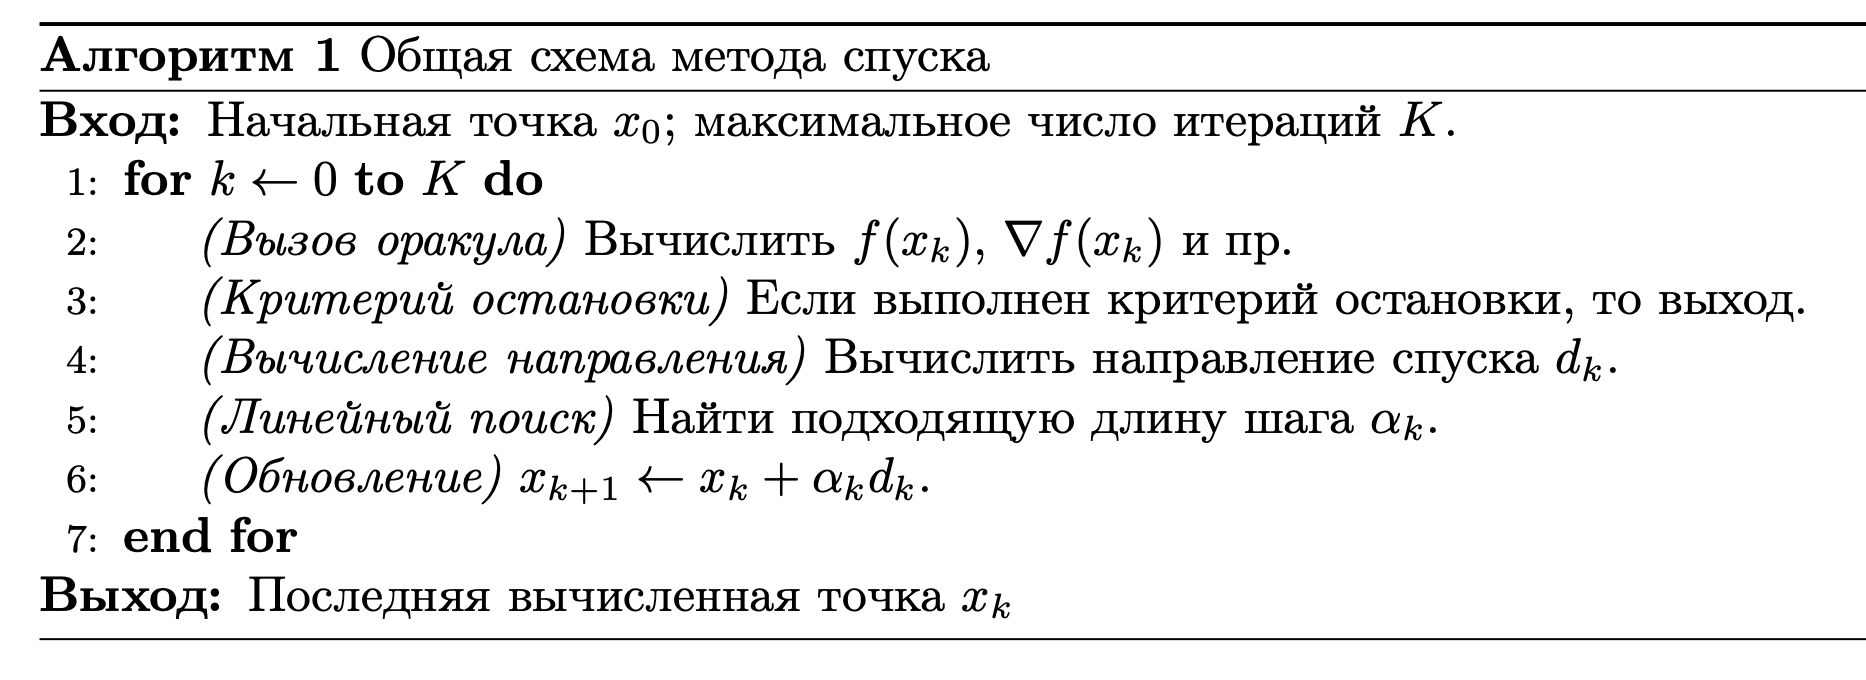
\includegraphics[width=16cm, height=6cm]{images/2-3-grad.png}
            \label{ris:im225}
            \caption{Метод спуска}
        \end{figure}

В случае градиентного спуска достаточно двух оракулов
$f(x_k)$ и
$\nabla f(x_k)$,
а в качестве направления  выбирается направление наискорейшего спуска:
$d_k = -\nabla f_k(x)$.

\subsubsection{Стратегии выбора длины шага
($\alpha_k$)}

Мы решаем подзадачу нахождения
$x_{k+1} = x_k - \alpha_k d_k$  в методе градиентного спуска. Нам бы хотелось найти такую точку $x_{k+1}$ которая бы давала значительное уменьшение целевой функции.
То есть наша задача состоит в минимизации функции
\begin{equation*}
    \phi_k(\alpha_k) = f(x_k + \alpha_k d_k)
\end{equation*}
Рассмотрим различные стратегии выбора длины шага:

\begin{enumerate}
    \item {\bf Последовательность
    $\{\alpha_k\}$ задана заранее.}

    Например:
    \begin{itemize}
        \item  $\alpha_k = \alpha > 0$ - константный шаг.
        Не гарантирует сходимость для всех гладких выпуклых функций. Сходимость гарантируется, если
        $\alpha \leqslant \frac{1}{L}$ и функция имеет липшицев градиент.
        \item  $\alpha_k = \frac{\alpha}{\sqrt{k+1}}$
        \item $\{\alpha_k\}$ такова,  что ряд
        $\sum \alpha_k$ расходится, а ряд $\sum \alpha_k^2$ сходится.         (ШАД 2019 Введение в методы оптимизации).
        Такие последовательности обеспечивают сходимость метода градиентного спуска для любых выпуклых гладких функций.
    \end{itemize}

    Применение:
    Очень простой метод, чаще всего применяется для задач выпуклой оптимизации.
    \item {\bf Полная релаксация} -
    $\alpha_k =  \argmin\limits_{\alpha > 0} f(x_k - \alpha \nabla f(x_k))$

    В этом случае можно использовать любые методы одномерной оптимизации, однако, точно эта задача обычно не решается.

    Применение:
    Имеет исключительно теоретический интерес, не применяется на практике.

    \item {\bf Бэктрекинг} - Метод дробления шага.
    Уменьшаем длину шага в фиксированное количество раз, пока не выполняется некоторое условие. В качестве условий часто применяются условия Армихо и Вульфа.

    Условие Армихо:
    $
        \phi_k (\alpha_k) \leqslant \phi_k(0) + c_1 \alpha \phi'_k(0), c_1 \in (0, 1)
    $

        Условия Вульфа:
    $
        \phi_k (\alpha_k) \leqslant \phi_k(0) + c_1 \alpha \phi'_k(0),
        \phi'_k (\alpha_k) \geqslant c_2 \alpha \phi'_k(0),
        0 < c_1 < c_2 < 1
    $

    Сильные условия Вульфа:

    \quad \quad $
        \phi_k (\alpha_k) \leqslant \phi_k(0) + c_1 \alpha \phi'_k(0),
        |\phi'_k (\alpha_k)| \leqslant c_2 \alpha |\phi'_k(0)|,
        0 < c_1 < c_2 < 1
    $


    \begin{figure}[H]
            \minipage{0.45\textwidth}
            \centering
            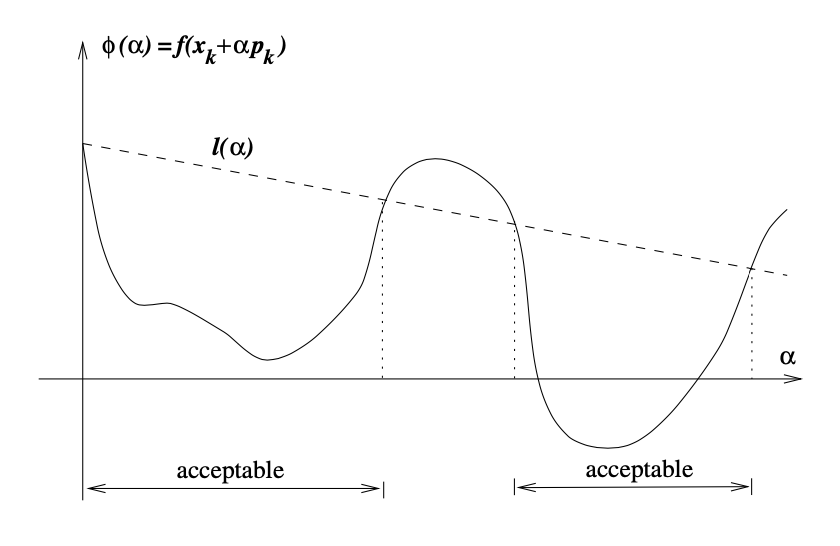
\includegraphics[scale=0.5]{images/2-3-armijo.png}
            \label{ris:im225}
            \caption{Иллюстрация к условию Армихо:
            Накладывает условие достаточного уменьшения функции.}
            \endminipage\hfill
            \minipage{0.45\textwidth}
            \centering
            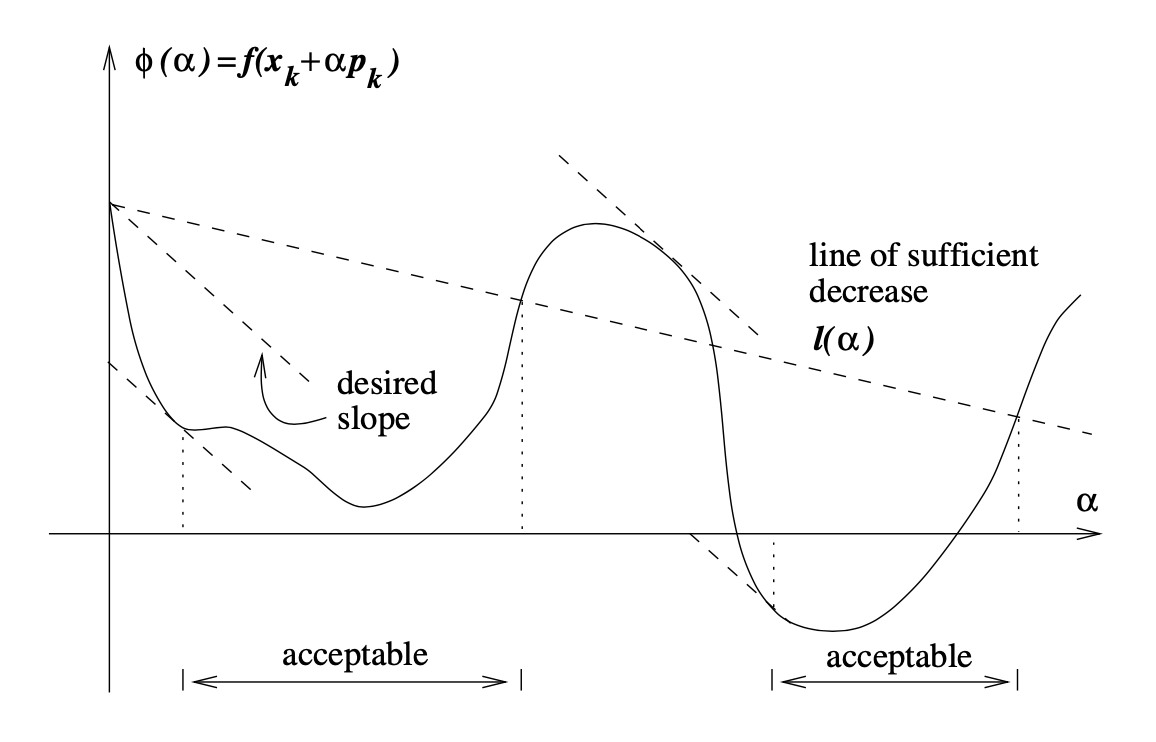
\includegraphics[scale=0.36]{images/2-3-wolfe.png}
            \label{ris:im225}
            \caption{Иллюстрация к условиям Вульфа: условие Армихо и
            условие кривизны функции: наклон не должен быть меньше начального, умноженного на константу.}
            \endminipage\hfill
    \end{figure}



    \begin{figure}[H]
            \centering
            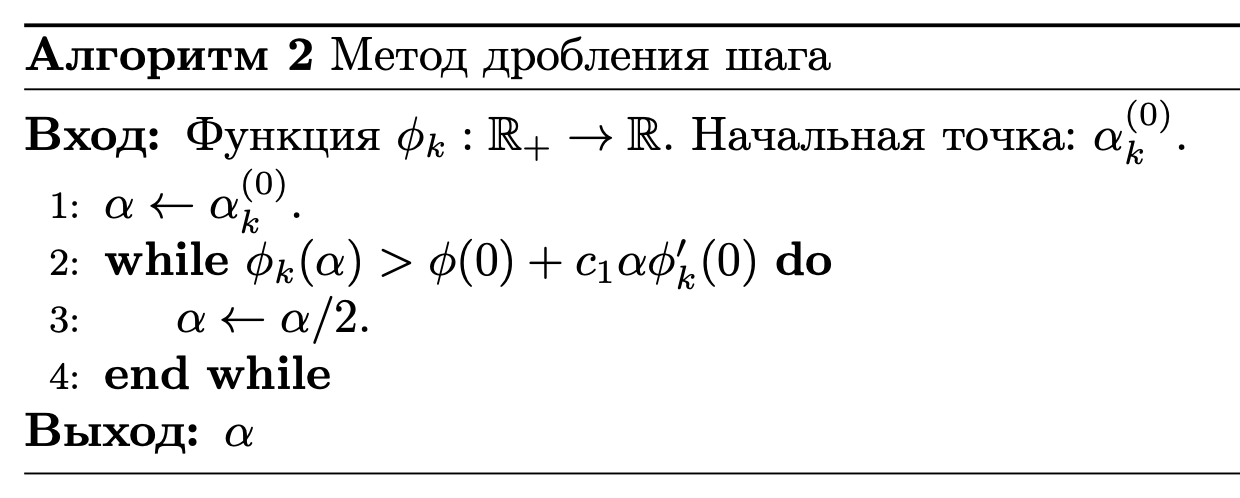
\includegraphics[width=16cm, height=6cm]{images/2-3-backtracking.png}
            \label{ris:im225}
            \caption{Процедура бэктрекинга с условием Армихо}
        \end{figure}


\end{enumerate}


\subsubsection{Скорость сходимости метода для сильно выпуклых функций }

{\bf Лемма 1}
Пусть
$f \in \mathscr{T}_{\mu, L}^{1,1}(\mathbb{R}^n)$.
Тогда
$\forall x, y \in \mathbb{R}^n$:

\begin{equation*}
    \langle
         \nabla f(x) - \nabla f(y), x-y
    \rangle
    \geqslant
    \frac{\mu L}{\mu + L} ||x-y||^2 +
    \frac{1}{\mu + L} ||\nabla f(x) - \nabla f(y)||^2
\end{equation*}

{\bf Лемма 2}
Пусть
$f \in \mathscr{F}_{L}^{1,1}(\mathbb{R}^n)$.
Тогда
$\forall x, y \in \mathbb{R}^n$:
\begin{equation*}
    0 \leqslant f(y) - f(x) -
    \langle
         \nabla f(x), y-x
    \rangle
    \leqslant \frac{L}{2} ||x-y||^2
\end{equation*}

{\bf Теорема (Скорость сходимости градиентного метода):}
Пусть
$f \in \mathscr{T}_{\mu, L}^{1,1}(\mathbb{R}^n)$,
$0 < h \leqslant \frac{2}{\mu + L}$.
Тогда градиентный метод с константным шагом $h$ образует такую последовательность
$\{x_k\}$, что
\begin{equation*}
    ||x_k - x^*||^2 \leqslant
    \left(
        1 - \frac{2h\mu L}{\mu + L}
    \right)^k
    ||x_0 - x^*||^2
\end{equation*}
При этом, если $h=\frac{2}{\mu + L}$,
обозначив
$Q_f = \frac{L}{\mu}$:
\begin{equation*}
    ||x_k - x^*|| \leqslant
    \left(
        \frac{Q_f - 1}{Q_f + 1}
    \right)^k
    ||x_0 - x^*||
\end{equation*}
\begin{equation*}
    f(x_k) - f^* \leqslant
    \frac{L}{2}
    \left(
        \frac{Q_f - 1}{Q_f + 1}
    \right)^{2k}
    ||x_0 - x^*||^2
\end{equation*}

{\bf Доказательство:}

Обозначим: $r_k = ||x_k - x^*||$.

\begin{align*}
r_{k+1}^2 = ||x_{k+1} - x^*||^2 = &
\Bigg [
    x_{k+1} = x_k - h \nabla f(x_k)
\Bigg]\\
= & ||x_k - x^* -  h \nabla f(x_k)||^2 =
\langle
    x_k - x^* -  h \nabla f(x_k), x_k - x^* -  h \nabla f(x_k)
\rangle = \\
=& r_k^2
- 2h \langle
    x_k - x^*, \nabla f(x_k)
\rangle
+ h^2 ||\nabla f(x_k)||^2 \leqslant
\Bigg [
    \text{Лемма 1}, \nabla f(x^*)=0
\Bigg]\\
\leqslant &
\left(
    1 - \frac{2h\mu L}{\mu + L}
\right)
r_k^2 +
h
\left(
    h - \frac{2}{\mu + L}
\right)
||\nabla f(x_k)||^2 \leqslant
\Bigg [
    h \leqslant \frac{2}{\mu + L}
\Bigg]\\
\leqslant &
\left(
    1 - \frac{2h\mu L}{\mu + L}
\right)
r_k^2  \leqslant
\Bigg [
   \text{индукция}
\Bigg]\\
\leqslant &
\left(
    1 - \frac{2h\mu L}{\mu + L}
\right)^{k+1}
||x_0 - x^*||^2
\end{align*}


Чтобы получить результаты при $h=\frac{2}{\mu + L}$,
необходимо подставить значение $h$ в формулу, получить первое неравенство и из него при помощи леммы 2 получить второе.


\begin{itemize}
    \item Отдельно отметим, что для класса
$\mathscr{F}_L^{p,k}(Q)$ у градиентного метода с константным шагом $\alpha = \frac{1}{L}$ сходимость  градиентного метода сублинейная.
\end{itemize}


\subsubsection{Примеры быстрой и медленной работы метода.}


Вспомним полученную нами скорость сходимости:

$Q_f = \frac{L}{\mu}$:
\begin{equation*}
    ||x_k - x^*|| \leqslant
    \left(
        \frac{Q_f - 1}{Q_f + 1}
    \right)^k
    ||x_0 - x^*||
\end{equation*}

Это означает, что скорость сходимости линейна, но зависит от $Q_f$, а именно, при $Q_f >> 1$ ($Q_f$ сильно больше 1) сходимость метода очень медленная: при $Q_f = 100 $:
$\frac{Q_f - 1}{Q_f + 1} \approx 0.98$,
$\left(
    \frac{Q_f - 1}{Q_f + 1}
\right)^{30} \approx 0.55$.


При $Q_f \approx 1$ сходимость метода быстрая: при $Q_f = 2 $:
$\frac{Q_f - 1}{Q_f + 1} = 0.33$,
$\left(
    \frac{Q_f - 1}{Q_f + 1}
\right)^{10} \approx 0.000015$.

Кроме того,
$Q_f$ - оценка числа обусловленности гессиана $f$.

\begin{itemize}
    \item  Число обучсловленности матрицы
$\mu(A) = ||A|| \times ||A^{-1}||$,     $||\cdot||$ - любая операторная форма - то есть число обусловленности зависит от выбора нормы.

Пример операторной нормы:
$||A|| = \max \{ ||Ax|| \text{ : } ||x|| = 1 \}$.
\end{itemize}


Получается, что чем ближе число обусловленности к 1, тем лучше работает метод.
В геометрическом смысле: при числе обусловленности, близком к 1, метод работает хорошо, а при больших числах обусловленности требуется сильно больше итераций:

В примерах $f(x) = \frac{1}{2} \langle Ax,x \rangle - \langle b,x \rangle$

\begin{figure}[H]
            \minipage{0.3\textwidth}
            \centering
            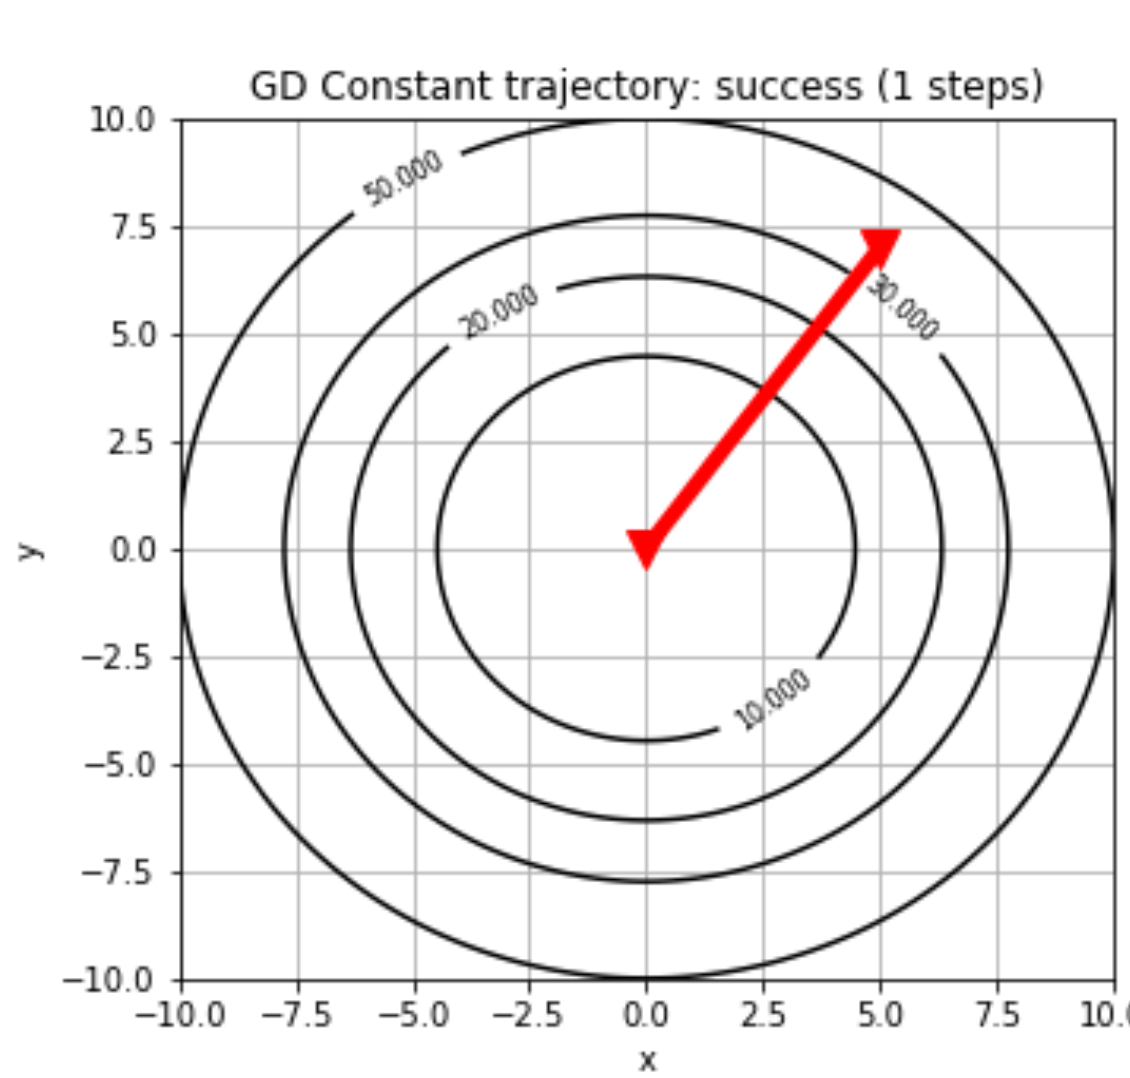
\includegraphics[scale=0.25]{images/2-3-traj1.png}
            \label{ris:im225}
            \caption{Число обусловленности $A$: 1}
            \endminipage\hfill
            \minipage{0.3\textwidth}
            \centering
            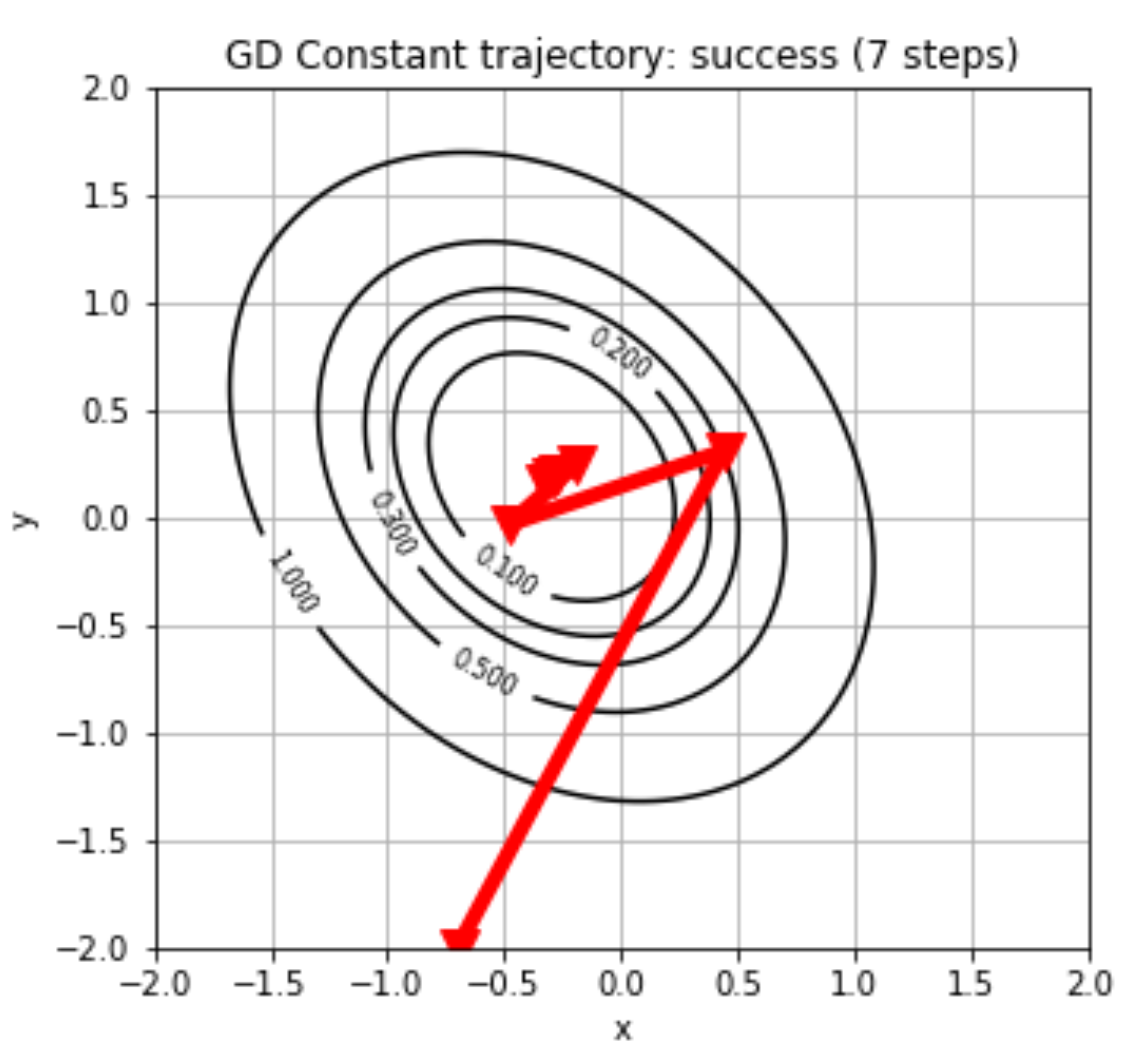
\includegraphics[scale=0.25]{images/2-3-traj2.png}
            \label{ris:im225}
            \caption{Число обусловленности $A$: 2}
            \endminipage\hfill
            \minipage{0.3\textwidth}
            \centering
            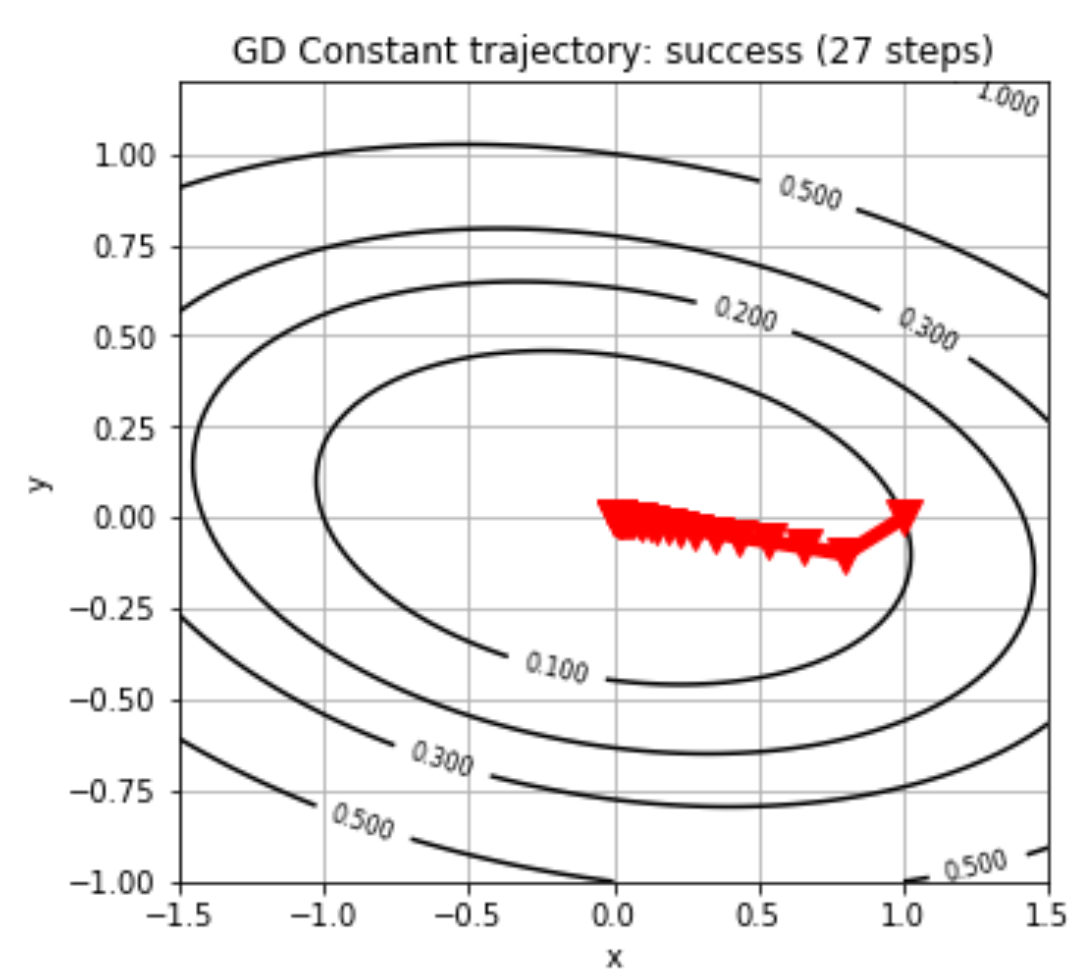
\includegraphics[scale=0.25]{images/2-3-traj6.png}
            \label{ris:im225}
            \caption{Число обусловленности $A$: 6.4}
            \endminipage\hfill
\end{figure}